\addtotoc{要旨（日本語）}
\thispagestyle{plain}

\vspace*{-6mm}
\begin{center}
\textbf{\large \titlenameJP}\\[1mm]
\end{center}

\begin{flushright}
\departmentnameJP\\
学生：\studentID, \authorShortJP\\
指導教員：\supervisornameJP
\end{flushright}

\vspace{1mm}
\setcounter{table}{0}
\setcounter{figure}{0}
\renewcommand{\thetable}{\arabic{table}}
\renewcommand{\thefigure}{\arabic{figure}}
\setlength{\columnsep}{7mm}
\begin{multicols}{2}
\setlength{\parskip}{5pt}
\sloppy

\noindent\textbf{1. 序論}

本研究は，多視点2D画像から完全自動化された3D再構成パイプラインおよびグラフィカルユーザーインターフェース（GUI）を開発し，マッチングパラメータが再構成精度に与える影響を実験的に評価することを目的とする。従来のStructure-from-Motion（SfM）およびMulti-View Stereo（MVS）手法は高い幾何学的精度を持つ一方で，計算コストが高く，パラメータの選択が出力品質に大きく影響する。

研究目的は：COLMAPおよびOpenMVSに基づく9段階パイプラインの構築；PyQt5ベースのGUIシステムの開発；マッチャー選択とマッチング戦略が精度に与える影響の実験的評価；Chamfer DistanceおよびRMSEによる再構成品質の測定；研究の限界の透明な記録。評価指標としてChamfer DistanceとRMSEを使用し，値が小さいほどグラウンドトゥルースに近い再構成を示す。

\noindent\textbf{2. 理論的背景と関連研究}

主要な先行研究として：Hartley \& Zisserman（2003）の多視点幾何学の理論的基礎；Lowe（2004）のSIFTによるスケール・回転不変な特徴検出；Sch{\"o}nberger \& Frahm（2016）のCOLMAPによるインクリメンタルSfMパイプライン；Cernea（2015）のOpenMVSによる密な再構成ツールキット。NeRF（Mildenhall et al., 2020）および3D Gaussian Splatting（Kerbl et al., 2023）はレンダリング品質に優れるが大量の計算リソースを必要とする。本研究では信頼性と将来的な機械学習統合の柔軟性を考慮し，従来のCOLMAP+OpenMVS手法を採用した。

\noindent\textbf{3. 研究方法と実装}

パイプラインはPythonで実装され（\texttt{core/}，\texttt{pipeline/}，\texttt{gui/}，\texttt{utils/}モジュール），PyQt5ベースのGUIはプログレスバー，リアルタイムログ出力，処理中断機能を提供する。ハードウェア：NVIDIA RTX 4060，Intel Core i9（第15世代），16\,GB RAM。

実験には3種類のデータセットを使用した（表~\ref{tab:summary_jp_datasets}）。Temple RingおよびCaterpillarデータセットは$1920\times1080$ JPEG解像度のオブジェクト写真で構成される。実験3では屋外の現実世界の再構成テストとして，公開されているLighthouse 4K動画（5:45，23.98\,fps，$4096\times2160$）を使用した（著者らが撮影したものではない）。

\begin{table}[H]
\centering
\caption{実験データセット}
\label{tab:summary_jp_datasets}
\scriptsize
\setlength{\tabcolsep}{3pt}
\begin{tabular}{|l|r|l|}
\hline
\textbf{データセット} & \textbf{画像数} & \textbf{使用実験} \\ \hline
Temple Ring & 47 & 実験1 \\ \hline
Caterpillar & 380${\sim}$ & 実験2 \\ \hline
Lighthouse 4K動画 & ${\sim}$86/172/200フレーム & 実験3 \\ \hline
\end{tabular}
\end{table}

3種類の実験を実施した：
\begin{itemize}
    \item \textbf{実験1：} SIFTとLightGlueのマッチャーを，exhaustiveおよびsequential（overlap=10）マッチング戦略と組み合わせた4構成をDataset Aで比較した。
    \item \textbf{実験2：} Sequentialマッチングのオーバーラップ値5，10，20，40をDataset Aで検証し，最適閾値を特定した。
    \item \textbf{実験3：} Lighthouse動画から4秒/2秒/1.5秒間隔でフレームを抽出した（${\sim}86$，${\sim}172$，${\sim}200$フレーム）。
\end{itemize}

\noindent\textbf{4. 研究結果と考察}

システムの主要性能指標：

\begin{table}[H]
\centering
\caption{主要性能指標}
\label{tab:summary_jp_results}
\scriptsize
\setlength{\tabcolsep}{3pt}
\begin{tabular}{|l|r|}
\hline
\textbf{指標} & \textbf{値} \\ \hline
Temple Ring（画像数） & 47 \\ \hline
スパース点群 & 35{,}000+点 \\ \hline
密な点群 & 210万点 \\ \hline
メッシュ頂点数/面数 & 120万/230万 \\ \hline
最良CD（1B：LG+Exhaustive） & 0.0074\,m \\ \hline
最良RMSE（1A：SIFT+Exhaustive） & 0.0064\,m \\ \hline
\end{tabular}
\end{table}

\textbf{実験1}では，マッチング戦略（exhaustive対sequential）の選択がマッチャー選択よりも精度に大きく影響することが示された。1Aと1Bはほぼ同等の結果を示したが，1D（LightGlue+Sequential）は壊滅的な失敗を示した--- overlap=10のsequentialマッチングは47枚のデータセットにおいてLightGlueに十分な対応点を生成できなかった。
\end{multicols}

\begin{figure}[H]
\centering
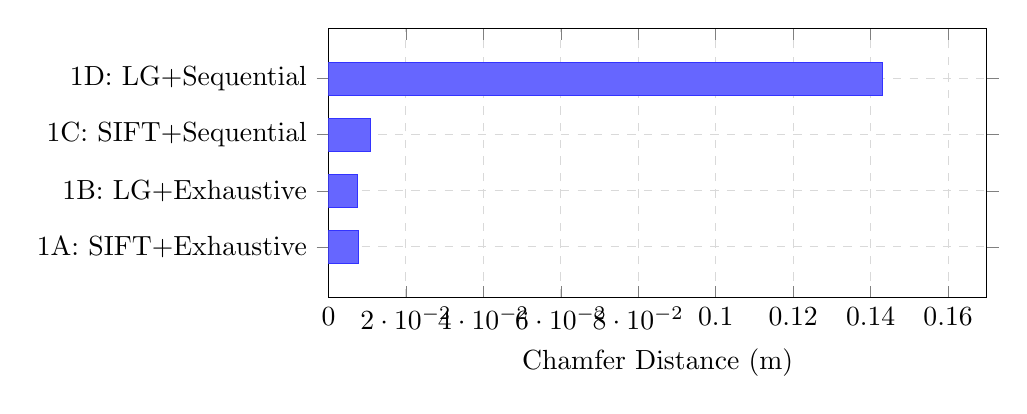
\begin{tikzpicture}
\begin{axis}[
    xbar, bar width=12pt,
    width=0.82\textwidth, height=5cm,
    symbolic y coords={1A,1B,1C,1D},
    ytick=data,
    yticklabels={
        {1A: SIFT+Exhaustive},
        {1B: LG+Exhaustive},
        {1C: SIFT+Sequential},
        {1D: LG+Sequential}},
    xlabel={Chamfer Distance (m)},
    xmin=0, xmax=0.17,
    enlarge y limits=0.3,
    grid=major, grid style={dashed,gray!30},
]
\addplot[fill=blue!60,draw=blue!80] coordinates {
    (0.007803,1A)(0.007437,1B)(0.010782,1C)(0.143084,1D)
};
\end{axis}
\end{tikzpicture}
\caption{実験1 --- マッチャーと戦略別Chamfer Distance比較}
\label{fig:jp_exp1_cd}
\end{figure}

\begin{figure}[H]
\centering
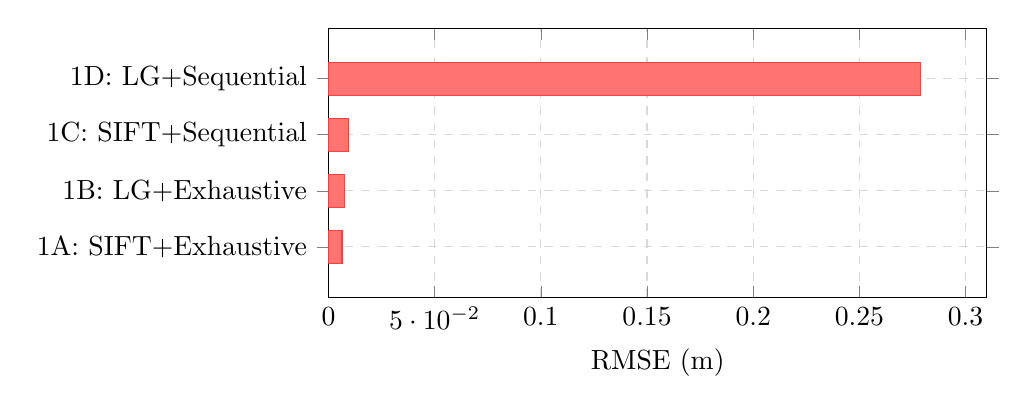
\begin{tikzpicture}
\begin{axis}[
    xbar, bar width=12pt,
    width=0.82\textwidth, height=5cm,
    symbolic y coords={1A,1B,1C,1D},
    ytick=data,
    yticklabels={
        {1A: SIFT+Exhaustive},
        {1B: LG+Exhaustive},
        {1C: SIFT+Sequential},
        {1D: LG+Sequential}},
    xlabel={RMSE (m)},
    xmin=0, xmax=0.31,
    enlarge y limits=0.3,
    grid=major, grid style={dashed,gray!30},
]
\addplot[fill=red!55,draw=red!75] coordinates {
    (0.006362,1A)(0.007368,1B)(0.009250,1C)(0.278657,1D)
};
\end{axis}
\end{tikzpicture}
\caption{実験1 --- マッチャーと戦略別RMSE比較}
\label{fig:jp_exp1_rmse}
\end{figure}

\begin{multicols}{2}

\textbf{実験2}では，sequentialオーバーラップに明確な閾値効果が確認された。overlap=5からoverlap=10への変更でChamfer Distanceが0.033\,m減少したが，10以上への増加では改善が無視できるほど小さかった。overlap=10がこのデータセット種別における最適設定として確認された。

\end{multicols}

\begin{figure}[H]
\centering
\begin{tikzpicture}
\begin{axis}[
    ybar, bar width=18pt,
    width=0.6\textwidth, height=5.5cm,
    symbolic x coords={5,10,20,40},
    xtick=data,
    xlabel={Sequentialオーバーラップ値},
    ylabel={誤差 (m)},
    ymin=0, ymax=0.18,
    enlarge x limits=0.2,
    legend style={at={(0.97,0.97)},anchor=north east,font=\small},
    grid=major, grid style={dashed,gray!30},
]
\addplot[fill=blue!60,draw=blue!80] coordinates {
    (5,0.152750)(10,0.119549)(20,0.120356)(40,0.119830)
};
\addplot[fill=red!55,draw=red!75] coordinates {
    (5,0.123995)(10,0.078579)(20,0.084193)(40,0.080573)
};
\legend{Chamfer Distance, RMSE}
\end{axis}
\end{tikzpicture}
\caption{実験2 --- Sequentialオーバーラップと誤差。overlap=5から10で品質が大幅改善，10以降の改善は微小。}
\label{fig:jp_exp2}
\end{figure}

\begin{multicols}{2}

\textbf{実験3}では，公開されているLighthouse 4K動画を屋外入力として使用した。重要な方法論的知見として，3Aの低いChamfer Distanceは優れた再構成品質を示すものではなく，参照点群サイズの18倍の差（95.2万対1,750万点）により構成間の直接比較が信頼できないことが明らかになった。比較可能な3Bと3Cでは，フレーム密度を高めるとChamfer Distanceが0.012\,m減少した。

\end{multicols}

\begin{figure}[H]
\centering
\begin{tikzpicture}
\begin{axis}[
    ybar, bar width=20pt,
    width=0.6\textwidth, height=5.5cm,
    symbolic x coords={3A (${\sim}$86),3B (${\sim}$172),3C (${\sim}$200)},
    xtick=data,
    xlabel={構成（フレーム数）},
    ylabel={誤差 (m)},
    ymin=0, ymax=0.095,
    enlarge x limits=0.2,
    legend style={at={(0.97,0.97)},anchor=north east,font=\small},
    grid=major, grid style={dashed,gray!30},
]
\addplot[fill=blue!60,draw=blue!80] coordinates {
    (3A (${\sim}$86),0.010333)
    (3B (${\sim}$172),0.053916)
    (3C (${\sim}$200),0.041948)
};
\addplot[fill=red!55,draw=red!75] coordinates {
    (3A (${\sim}$86),0.017397)
    (3B (${\sim}$172),0.082545)
    (3C (${\sim}$200),0.066822)
};
\legend{Chamfer Distance, RMSE}
\end{axis}
\end{tikzpicture}
\caption{実験3 --- フレームサンプリングと誤差（Lighthouse 4K動画）。参照点群サイズの18倍の差により3Aと3B/3Cの直接比較は無効。}
\label{fig:jp_exp3_errors}
\end{figure}

\begin{figure}[H]
\centering
\begin{tikzpicture}
\begin{axis}[
    ybar, bar width=20pt,
    width=0.6\textwidth, height=4.5cm,
    symbolic x coords={3A (${\sim}$86),3B (${\sim}$172),3C (${\sim}$200)},
    xtick=data,
    xlabel={構成（フレーム数）},
    ylabel={参照点数（百万）},
    ymin=0, ymax=24,
    enlarge x limits=0.2,
    grid=major, grid style={dashed,gray!30},
]
\addplot[fill=teal!55,draw=teal!75] coordinates {
    (3A (${\sim}$86),0.952)
    (3B (${\sim}$172),17.468)
    (3C (${\sim}$200),21.452)
};
\end{axis}
\end{tikzpicture}
\caption{実験3 --- 参照点群サイズ。3Aと3B/3Cの18倍の差により指標の直接比較は無効。}
\label{fig:jp_exp3_pts}
\end{figure}

\begin{multicols}{2}

以下の限界点を記録する：
\begin{itemize}
    \item テストした物体の種類が1種類のみであり（実験1・2），汎化性能は未確認，
    \item 実験3の参照点群サイズの不均等により，構成間の比較が信頼できない，
    \item GUIにカメラキャリブレーションインターフェースが不足，
    \item Sequentialマッチングは小規模データセットで一部のマッチャーに失敗する。
\end{itemize}

工学的観点から，本研究はデータ収集からスパース・密再構成，メッシュ生成，テクスチャマッピングまでの全再構成パイプラインをPyQt5 GUIシステムに統合した。今後の研究では，SuperPoint/SuperGlueおよびLightGlueの統合，NeRFおよびGaussian Splattingとの比較，多様な物体カテゴリへの評価拡張が重要な課題となる。

\noindent\textbf{5. 参考文献}

\small
\begin{enumerate}
\setlength{\itemsep}{1pt}\setlength{\parsep}{0pt}\setlength{\topsep}{2pt}
    \item Hartley, R., \& Zisserman, A. (2003). \textit{Multiple View Geometry in Computer Vision}. Cambridge University Press.
    \item Lowe, D. G. (2004). Distinctive image features from scale-invariant keypoints. \textit{IJCV}, 60(2), 91--110.
    \item Sch{\"o}nberger, J. L., \& Frahm, J. M. (2016). Structure-from-motion revisited. \textit{CVPR}, 4104--4113.
    \item Cernea, D. (2015). OpenMVS: Multi-View Stereo Reconstruction Library.
    \item Mildenhall, B., et al. (2020). NeRF: Representing scenes as neural radiance fields. \textit{ECCV}, 405--421.
    \item Lindenberger, P., et al. (2023). LightGlue: Local feature matching at light speed. \textit{ICCV}, 17627--17638.
\end{enumerate}
\normalsize

\end{multicols}
